\documentclass[11pt]{article}

\usepackage[utf8]{inputenc}
\usepackage[ngerman]{babel}
\usepackage[hyphens]{url}
\usepackage{hyperref}
\usepackage{graphicx}
\usepackage{float}
\usepackage{courier}

\usepackage[normalem]{ulem}
\usepackage{listings}
\usepackage{xcolor}
\usepackage{graphicx}
\usepackage{subcaption}


%% Custom Listen für die Anforderungen
\usepackage{enumitem}

\newlist{FA}{enumerate}{1}
\setlist[FA]{label=FA-\arabic*:,leftmargin=*, align=left, labelindent=0.6cm}

\newlist{NFA}{enumerate}{1}
\setlist[NFA]{label=NFA-\arabic*:,leftmargin=*, align=left, labelindent=0.6cm}


%% ER Diagramm
\usepackage{tikz}
\usetikzlibrary{er,positioning}



%%%%%%%%%%%%%%%%%%%%%%%%%%%%%%%%%%%%%%%%%%

\title{Dokumentation der App "Copypasta"}
\author{Tanja Noack, Janine Kostka}
\date{\today}

%%%%%%%%%%%%%%%%%%%%%%%%%%%%%%%%%%%%%%%%%%

\begin{document}
	\begin{titlepage}
		\centering
		\maketitle
		\thispagestyle{empty}
		\textcolor{red}{\textbf{{\LARGE \#TODO}}}
		
		\vspace{2cm}
		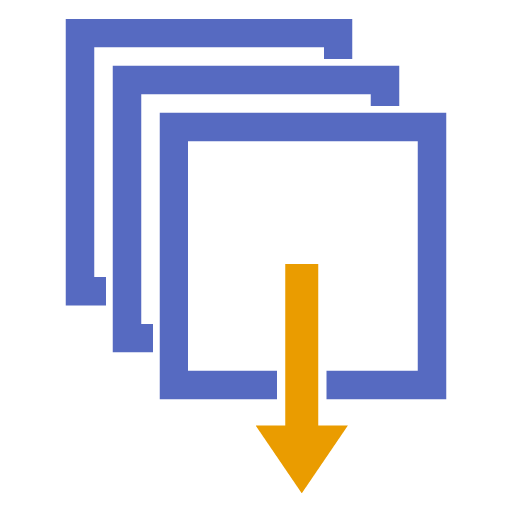
\includegraphics[width=0.3\textwidth]{Konzepte/logo.png}\par\vspace{1cm}
		
		\vfill
	\end{titlepage}
	\pagebreak
	
	%%%%%%%%%%%%%%%%%%%%%%%%%%%%%%%%%%%%%%%%%%
	
	\tableofcontents
	\pagebreak
	
	%%%%%%%%%%%%%%%%%%%%%%%%%%%%%%%%%%%%%%%%%%
	
\section*{To-Do}
	\begin{itemize}
		\item Deckblatt bisschen verschönern
		\item Einleitung schreiben
		\item Code listings etwas besser aussehen lassen (listings-Package konfigurieren)
	\end{itemize}

\section*{Anmerkungen (braucht ne bessere Überschrift)}
	Releases sind unter \sloppy\url{https://github.com/qn0x/copypasta/releases} zu finden. Dort befindet sich eine Option zum Herunterladen der APK.  
	Des Weiteren wird der Quellcode über Github unter \sloppy\url{https://github.com/qn0x/copypasta} gehostet. \\
	Die im Weiteren Verlauf der Dokumentation abgebildeten Screenshots stammen aus dem Release v0.1.

\section{Einleitung}
	Warum haben wir dieses Thema ausgewählt? Du hast da ne ganz gut Einleitung während der Präsentation gemacht, weiß leider nicht mehr so genau was genau darin vorkam.\\
	\textcolor{red}{\textbf{{\LARGE \#TODO}}}
	

\section{Anforderungen}
	Das Projekt besteht aus zwei Komponenten:
	\begin{enumerate}
		\item einer App, um Textschnipsel zu organisieren und die Tastatur zu konfigurieren, sowie
		\item einer Tastatur, die ihren Inhalt je nach Einstellung des Benutzers verändert und beim Tippen auf den entsprechenden Button den Inhalt des Textschnipsels in das aktive Eingabefeld einfügt.
	\end{enumerate}
	\subsection{Funktionale Anforderungen}
		\subsubsection{App}
		\begin{FA}
			\item Die Textschnipsel bestehen jeweils aus Text, Name bzw. Titel des Schnipsels und einer Liste von Tags.
			\item Alle vorhandenen Textschnipsel werden als Liste innerhalb der MainActivity angezeigt.
			\item Der Benutzer soll eigene Textschnipsel abspeichern, löschen und verändern können.
			\item Der Benutzer kann nach Textschnipseln suchen. Dabei soll die Suchfunktion folgende Methoden unterstützen:
				\begin{enumerate}
					\item Volltextsuche. Dabei sollen die abgespeicherten Texte nach den im Suchfeld eingegebenen Text durchsucht werden.
					\item Tagsuche. Mit Setzen eines '\#' zu Beginn der Sucheingabe soll nach vorhandenen Tags gesucht werden.
					\item Titelsuche. Mit Setzen eines '@' zu Beginn der Sucheingabe soll nach vorhandenen Titeln gesucht werden
				\end{enumerate}
			\item Der Benutzer soll zur Laufzeit der App selbst festlegen können welche Textschnipsel auf der Tastatur angezeigt werden. 
		\end{FA}
		
		\subsubsection{Tastatur}
		\begin{FA}[resume]
			\item Die Tastatur soll als Anzeige von als Favorit markierten Textschnipseln dienen. Diese werden in Form von Buttons dargestellt.
			\item Die Anzeige der Textschnipsel soll mittels deren Namen bzw. Titel als Label auf Buttons erfolgen.
			\item Änderungen des Favoritenstatus innerhalb der App sollen zur Laufzeit beim nächsten Sichtbarwerden der Tastatur widergespiegelt werden.
			\item Beim Tippen auf einen Button auf der Tastatur soll der Inhalt des auf dem Button angezeigten Textschnipsels in das aktive Eingabefeld eingefügt werden.
			\item Mit einem Swipe Left soll der zuletzt eingefügte Text wieder gelöscht werden.
			\item Es sollen pro Zeile der Tastatur genau vier Buttons dargestellt werden. 
			\item Die Anzahl der Zeilen ist auf maximal vier begrenzt.
			\item Zeilen sollen je nach Anzahl der Favoriten ein- bzw. ausgeblendet werden. So sollen beispielsweise bei vier Favoriten genau eine Zeile und bei fünf Favoriten zwei Zeilen dargestellt werden.
		\end{FA}

	\subsection{Nichtfunktionale Anforderungen}
		\begin{NFA}
			\item Aussehen und Handhabung. Die App soll im Android-Standarddesign gehalten sein, damit sich neue Benutzer schnell zurechtfinden.
			\item Benutzbarkeit. Die Oberfläche soll schlicht sein. Wenige Elemente, um die Bedienbarkeit und Erlernbarkeit zu gewährleiste.
			\item Schnelligkeit. Der Nutzer soll in keinem Fall nach einer Aktion innerhalb der App mehr als 2 Sekunden auf eine Antwort waren müssen.
			\item Korrektheit. Es sollen keine Anzeigefehler auf den getesteten Geräten auftauchen.
			\item Weiterentwicklungsmöglichkeiten. Die Implementierung soll es ermöglichen einfach die Funktionalität der App zu erweitern.
		\end{NFA}
	
	
\section{Architektur und Implementierung}
	Welche Frameworks wurden benutzt? Welche Zusammenhänge sind zwischen den Modulen etc.?\\
	Grundsätzlich erfolgt eine Trennung der App und der Tastatur und zwei unabhängige Einheiten.
	Eine Kommunikation zwischen beiden ist nicht vorgesehen.
	Um dennoch die in der App als Favoriten markierten Textschnipsel auf der Tastatur anzeigen zu können wird die gleiche Datenquelle von beiden Einheiten benutzt.
	Als gemeinsame Datenquelle wird die von der Android-Runtime angebotene SQLite-Datenbank benutzt.
		
		\subsection{Persistence Layer - SQLite-Datenbank mit Room-Framework}
			Für die persistente Speicherung der Textschnipsel wird die SQLite Datenbank genutzt. 
			Um unnötigen Aufwand bei CRUD-Operationen(Create, Read, Update, Delete) zu sparen wird das  bereitgestellte Framework Room genutzt. \newline
			Abbildung \ref{fig:room_arch} zeigt eine grobe Übersicht der Architektur der Objektrelationalen Modellierung. Letztlich werden werden als Entity definierte Klassen in der Datenbank als jeweils eigene Tabelle gespeichert. Jegliche Zugriffe und Operationen auf die Datenbank erfolgen über sogenannte Data Access Objects (DAO). 
						
			\begin{figure}[H]
				\centering
				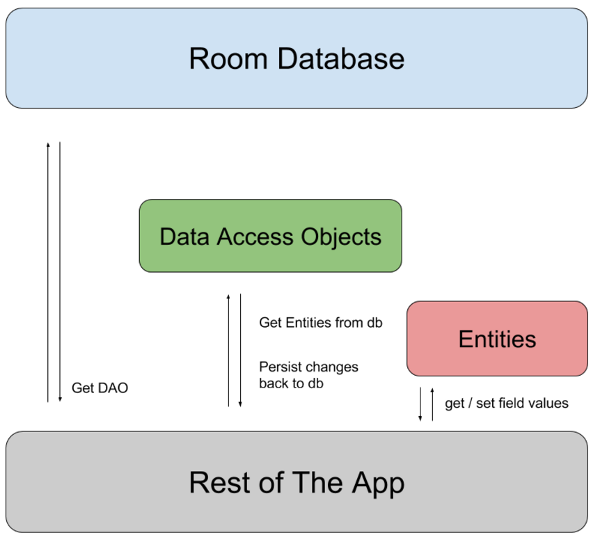
\includegraphics[width=0.8\textwidth]{Konzepte/room_architecture.png}
				\caption{\href{https://developer.android.com/training/data-storage/room/}{Architektur}}
				\label{fig:room_arch}
			\end{figure}
		
			\noindent Im Falle der App zusätzlich ein Repository mit einem ViewModel wie in Abbildung \ref{fig:room_vm} verwendet. Dies ermöglicht eine Erweiterung der Datenquellen. Als weitere Datenquelle könnten beispielsweise die Antworten einer API dienen. Für die Oberfläche sehen diese weiteren Daten dann gleich aus wie die Daten aus der Datenbank.
			
			\noindent Da für die Tastatur jeweils nur eine Anfrage (alle Favoriten ausgeben) an die Datenbank gemacht wird, wird auf das Repository und das ViewModel verzichtet.
			
			\begin{figure}[H]
				\centering
				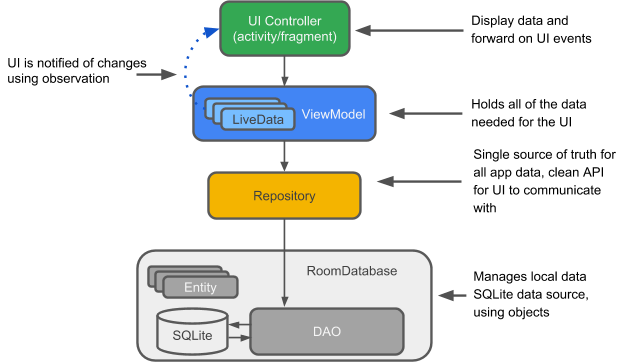
\includegraphics[width=\textwidth]{Konzepte/room_viewmodel.png}
				\caption{\href{https://codelabs.developers.google.com/codelabs/android-room-with-a-view/}{Room-Architektur mit ViewModel}}
				\label{fig:room_vm}
			\end{figure}
			
			\noindent Es werden 3 Tabellen verwendet, welche das in Abbildung \ref{fig:er} dargestellte ER-Modell abbilden.\medskip
			
			\begin{figure}[H]
				\begin{tikzpicture}[auto,node distance=1.5cm]
					\node[entity] (node1) {Snippet}
					[grow=up,sibling distance=2.2cm]
					child {node[attribute] {\underline{ID}}}
					child {node[attribute] {Name}}
					child {node[attribute] {Favorite}}
					child[grow=left,level distance=2.2cm] {node[attribute] {Text}};
					
					% Now place a relation (ID=rel1)
					\node[relationship] (rel1) [below right = of node1] {Assign};
					
					% Now the 2nd entity (ID=rel2)
					\node[entity] (node2) [above right = of rel1]	{Tag}
					[grow=up,sibling distance=2.2cm]
					child[grow=right,level distance=3cm] {node[attribute] {\underline{Name}}};
					
					% Draw an edge between rel1 and node1; rel1 and node2
					\path (rel1) edge node {} (node1)
					edge	 node {}	(node2);
				\end{tikzpicture}
				
				\label{fig:er}
				\caption{ER-Modell in der SQLite Datenbank}
			\end{figure}
			
		
		\subsection{App}
			Die App besteht aus insgesamt drei verschiedenen Activites - der MainActivity, der NewSnippetActivity und der ViewSnippetActivity, in Abbildung \ref{fig:activities} zu sehen sind. 
			
			\begin{figure}
				\centering
				\begin{subfigure}[b]{0.3\textwidth}
					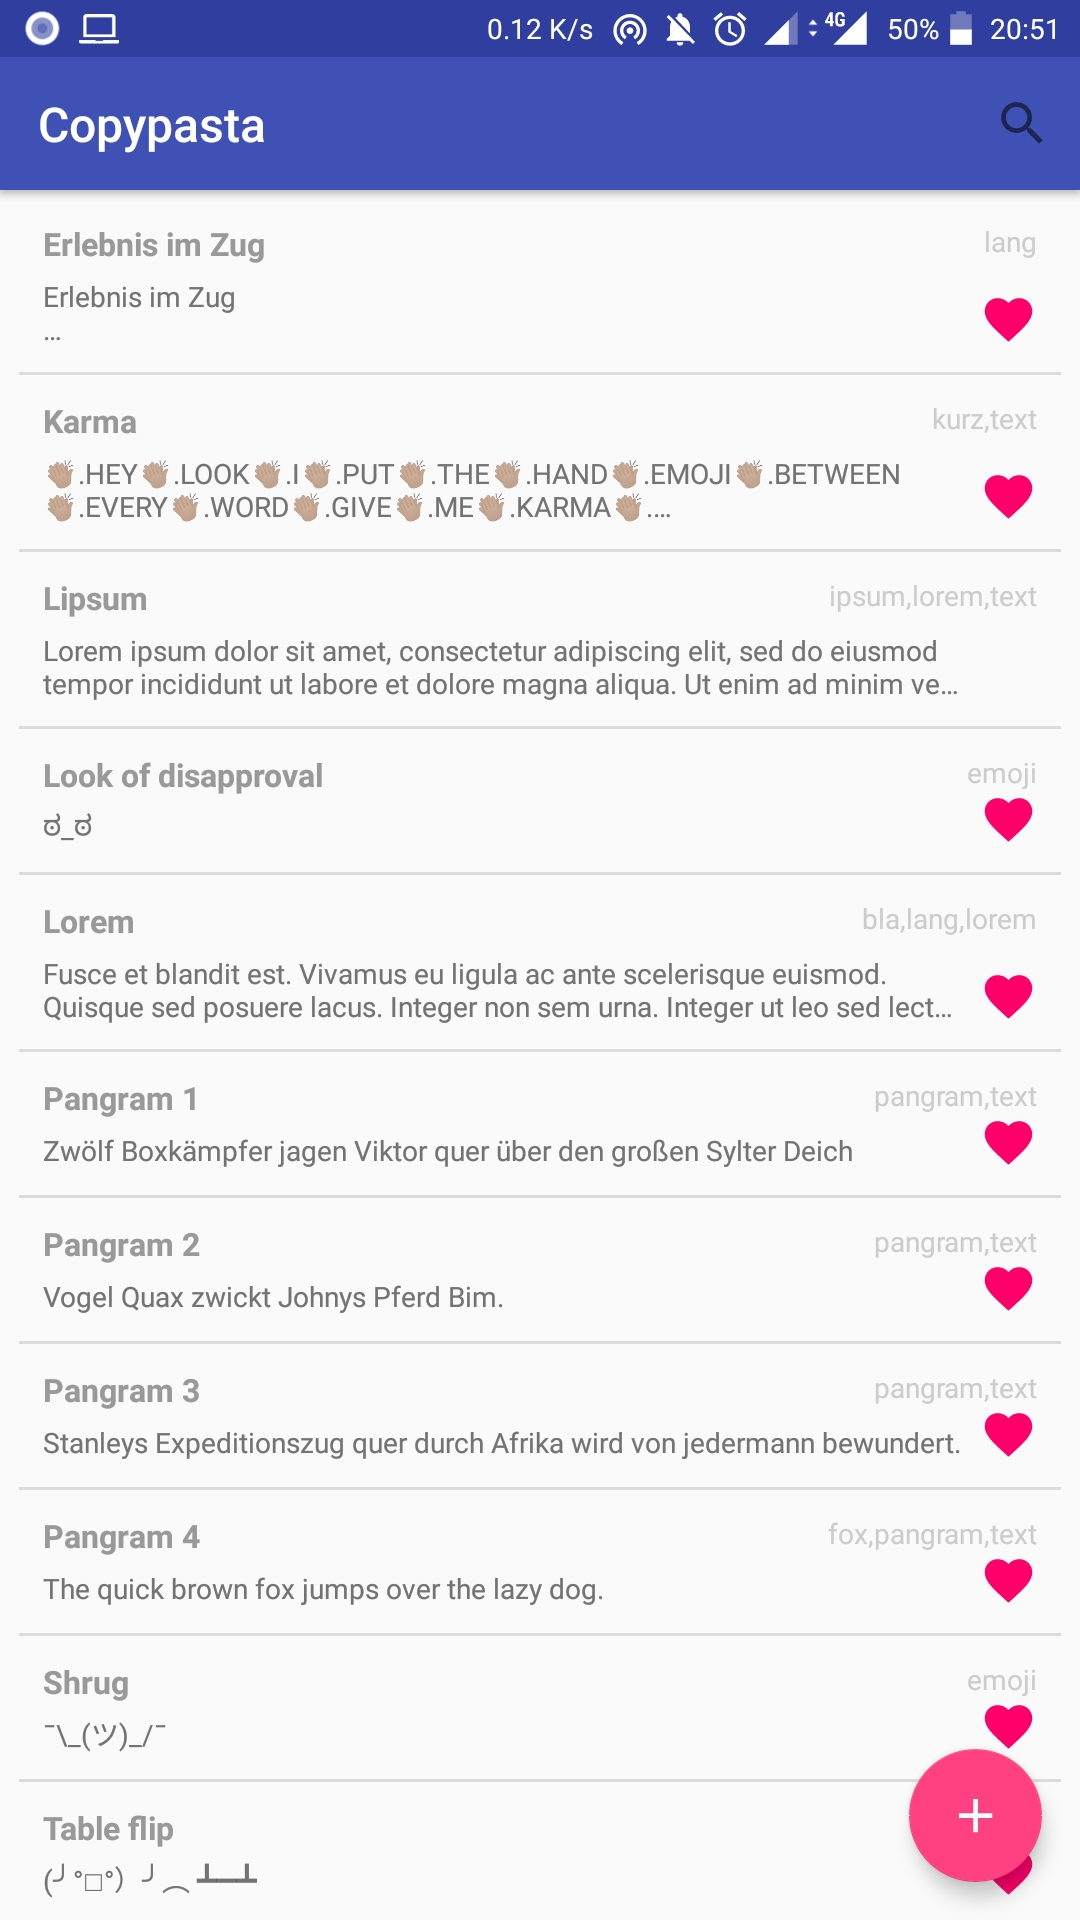
\includegraphics[width=\textwidth]{Konzepte/screenshots/main_list.jpg}
					\caption{MainActivity}
				\end{subfigure}
				~ %add desired spacing between images, e. g. ~, \quad, \qquad, \hfill etc. 
				%(or a blank line to force the subfigure onto a new line)
				\begin{subfigure}[b]{0.3\textwidth}
					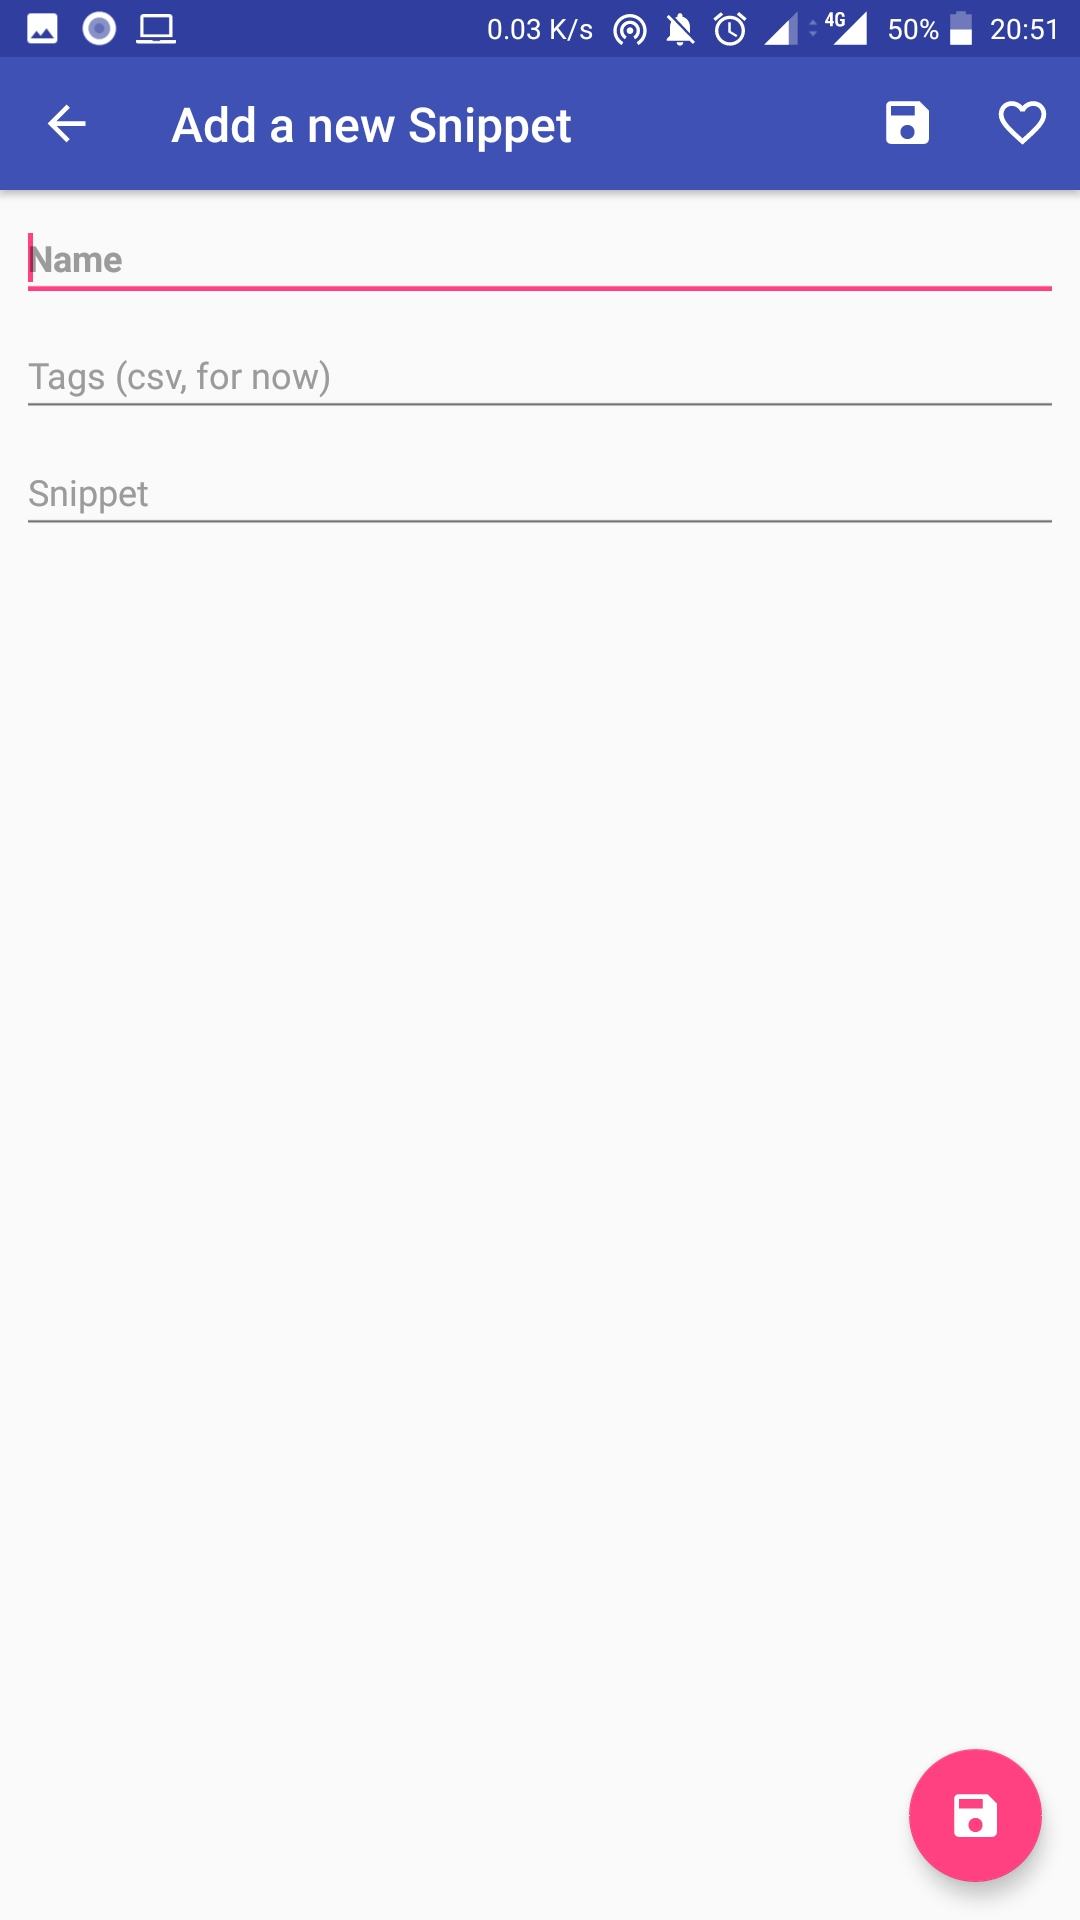
\includegraphics[width=\textwidth]{Konzepte/screenshots/add_snippet.jpg}
					\caption{NewSnippetActivity}
				\end{subfigure}
				~ %add desired spacing between images, e. g. ~, \quad, \qquad, \hfill etc. 
				%(or a blank line to force the subfigure onto a new line)
				\begin{subfigure}[b]{0.3\textwidth}
					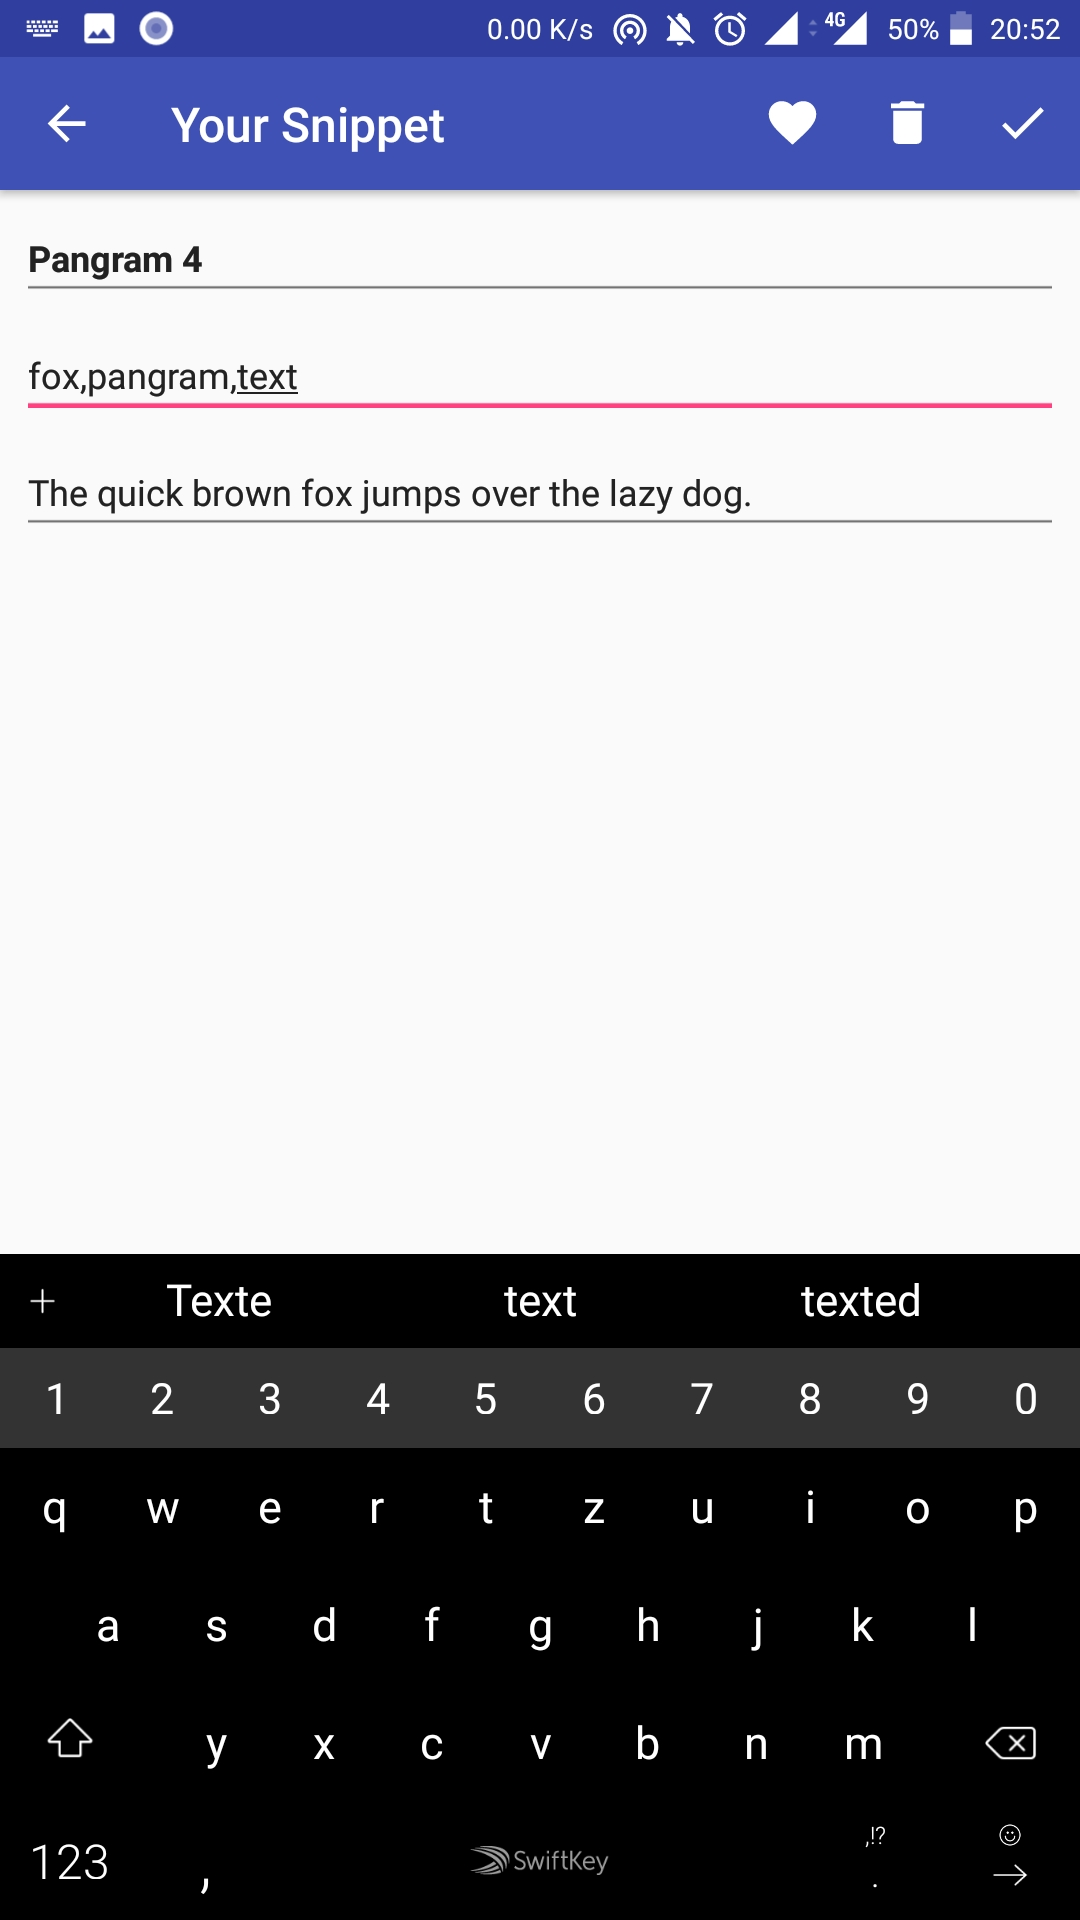
\includegraphics[width=\textwidth]{Konzepte/screenshots/edit_snippet.jpg}
					\caption{ViewSnippetActivity}
				\end{subfigure}
				\caption{Scrennshots der drei Activities der App}
				\label{fig:activities}
			\end{figure}
		
			\subsubsection{MainAcitivity}
				Kurz beschreiben blabla \\
				\textcolor{red}{\textbf{{\LARGE \#TODO}}}
				
			\subsubsection{NewSnippetActivity}
				\textcolor{red}{\textbf{{\LARGE \#TODO}}}
			
			\subsubsection{ViewSnippetActivity}
				\textcolor{red}{\textbf{{\LARGE \#TODO}}}
		
		
		\subsection{Tastatur}
			\noindent Für die Tastatur soll eine eigene sogenannte InputMethod mittels der bereitgestellten \href{https://developer.android.com/guide/topics/text/creating-input-method.html}{API} implementiert werden. Statt den einzelnen Tasten sollen dann Inhalte aus der App angezeigt werden, die vom Nutzer selbst festgelegt werden können.\\
		
			\noindent Die angepasste Tastatur ist als eine zusätzliche, normale Android Systemtastatur implementiert worden. Dabei gliedert sich der Aufbau wie folgt: 
			\begin{itemize}
				\item \texttt{xml/keyboard.xml} enthält die Aufteilung der Tastatur, wie diese in \texttt{Keyboard.Row} und \texttt{Keyboard.Key} unterteilt ist
				\item \texttt{xml/method.xml} Festlegen der InputMethod als Systemtastatur
				\item \texttt{layout/keyboard\_view.xml} ist das Layout der Tastatur, welches aufgerufen wird
				\item \texttt{layout/key\_preview.xml} dient der Key-Popup-Funktion, falls ein Key mehrere Symbole ausgeben kann. In unserem Fall wird diese nicht genutzt.
				\item \texttt{SnippetInputService.java} ist die Javaklasse, in welcher die Keyboardfunktionen implementiert wurden, zum Beispiel das Instanzieren des Keyboards, Laden der Snippets aus der Datenbank und entsprechendes Einfügen auf die Knöpfe der Tastatur
			\end{itemize}
		
			\subsubsection{Extended InputMethodService}
				Für die Tastatur wird der von Android definierte InputMethodService erweitert. \\
				Beschreibung der Klasse SnippetInputService, wie diese Daten aus der DB zieht, die Label und OutputText der Buttons setzt, wie das Layout der Tastatur über die verschiedenen XML-Ressourcen definiert wird.
		
	
\section{Probleme und deren Lösung}
	Falls wir noch Prosa schreiben müssen könnten wir hier auch verworfene Ideen aus den Notizen unten aufführen.
	\subsection{Speicherung der Textschnipsel}
		Es wurde aus drei Möglichkeiten eine ausgewählt, die im \href{https://developer.android.com/guide/topics/data/data-storage}{Developer-Guide} zu finden sind.
		\begin{enumerate}
			\item Im Dateisystem speichern. Hierfür müsste ein bestimmtes Format, z.B. JSON gewählt werden. Die Datei müsste hierbei häufig gelesen und beschrieben werden, was zusätzlichen Aufwand bei der Implementierung und verringerte Responsivität bei vielen Textschnipseln nach sich zieht.
			\item Im Key-Value-Store speichern. Es können nur primitive Datentypen gespeichert werden. Somit müsste wiederum ein Format gewählt werden, welches die Textschnipsel in einem primitiven Datentyp darstellt, z.B. als JSON-String. Dies führt dazu, dass diese (De-)serialisiert und geparst werden müssten. Somit ergibt sich wie beim Speichern als "einfache" Datei ein zusätzlicher Aufwand.
			\item In der Datenbank speichern. Beim Initialisieren erfordert diese Lösung durch die Konfiguration der Datenbank mehr Aufwand. Bei einer großen Menge an Textschnipseln bietet eine Datenbank deutlich bessere Performance, sowie einfachere Migration und Erweiterung bei eventuell auftretenden Änderungen am Datenbankschema. Zusätzlich bietet die Android-Laufzeitumgebung das Framework Room, welches die manuelle Kommunikation mit der Datenbank noch mehr vereinfacht und übersichtlicher macht.
		\end{enumerate}
		Nach Abwägung dieser Möglichkeiten wurde die Lösung mit der Datenbank ausgewählt. Zwar wird für die Einarbeitung für die Nutzung der Datenbank mehr Zeit benötigt aber die oben genannten Vorteile überwiegen die wenigen Nachteile.
	
		\subsubsection{Persistenz mit Room-Library}
			Die Textschnipsel sollten in der nativen SQLite-Datenbank gespeichert werden. Wie im Teil der Archtitektur schon beschrieben, werden diese in insgesamt drei Tabellen gespeichert. Diese bilden eine Many-to-many-Relation auf der Datenbankebene ab. Room bietet aber nur Annotationen für One-to-Many Relationen. Dementsprechend musste entsprechend zusätzlich ein DAO für diese Hilfstabelle erstellt werden. \\
			Asynchrone Operationen blabla \textcolor{red}{\textbf{{\LARGE \#TODO}}}
			
			
	\subsection{Custom Keyboard}
		Für die Erstellung einer für die Zwecke der App angepassten Tastatur gab es Vorüberlegungen und Ideen, welche später durch mangelnde Möglichkeiten verworfen werden mussten. Dazu zählen unter anderem: 
		\begin{itemize}
			\item Anzeige der (kompletten) Liste an Snippets 
			\item Autovervollständigung: Ab dem Eintippen wird die Liste aktualisiert mit allen Einträgen, die mit der Eingabe beginnen oder sie enthalten
			\item Häufigkeitsanalyse: Anzeige der häufig genutzten Snippets an erster Stelle
			\item Einbinden der Liste der Snippets in Tastatur durch einen extra Menüpunkt: Layout einer normalen Systemtastatur, allerdings mit einem zusätzlichen Button, um auf die Snippets zugreifen zu können
		\end{itemize}
		
		Des Weiteren gab es bei der Implementierung der bestehenden Tastatur Probleme, welche bei der Weiterentwicklung berücksichtigt werden sollten:
		\begin{itemize}
			\item nur outdated Tutorials gefunden
			\item Doku eher unvollständig
			\item Bsp: android:codes akzeptiert laut Doku Strings mit Unicode Charaktern, in der Implementierung werden aber nur Int-Codes akzeptiert
			\item nach einigem Suchen herausgefunden, dass Strings mittels android:keyOutPutText eingefügt werden können. Diese werden nicht über onKey, sonder über onText eingefügt.
		\end{itemize}
		\subsubsection{Definition des Tastaturlayouts}
			Lösung über mehrere XML-Definition, die jeweils die gewünschte Anzahl der Reihen enthalten. Berechnung bei \lstinline|onStartInputView()|, also bei jedem Sichtbarwerden der Tastatur.\textcolor{red}{\textbf{{\LARGE \#TODO}}}
	
\section{Ausblick}
	Was gibt es, was später noch eingebaut werden könnte?
	\begin{itemize}
		\item receive text from other apps via sharing
		\item Häufigkeitsanalyse: wird viel benutzt -> wird als erstes angezeigt
		\item Mehr Einstellungsmöglichkeiten für 
	\end{itemize}
	
	
\section{Wer hat was gemacht?}
	Janine alles, Tanja nix.
	Da ichs nie auf die Reihe kriegen werde das persönlich zu sagen, weil ich viel zu awkward für so etwas bin.. es tut mir so Leid, dass ich mich von dir so hab durchs Semester ziehen lassen. Jedes Mal, wenn ich versucht habe etwas anzufangen, ging es einfach nicht, weil mein Kopf sonstwo steckt. Ich bekomme derzeit nichts auf die Reihe außer Kleinigkeiten und selbst bei denen versage ich regelmäßig.
	Danke, dass du es erträgst. Danke, dass du mir hilfst. Danke, dass du mich so durchziehst. \bigskip\\
	Janine: App\\
	Tanja: Tastatur\\
	Denke, das passt dann so :)

	
	
	%%%%%%%%%%%%%%%%%%%%%%%%%%%%%%%%%%%%%%%%%%
\end{document}
